\documentclass{article}
\usepackage[utf8]{inputenc}
\usepackage[T1]{fontenc}
\usepackage[utf8]{inputenc}
\usepackage{graphicx}
\usepackage[a4paper, total={6.5in, 8.6in}]{geometry}
\setcounter{secnumdepth}{4}
\usepackage{hyperref}
\usepackage{color}
\usepackage{booktabs}
\usepackage{tabularx}
\usepackage{amsmath}
\usepackage{textcomp}
\usepackage{xcolor}
\usepackage{listings}
\usepackage{enumitem}
\usepackage{minted}
\usepackage{tikz}
\usepackage{ccicons}
\usepackage{fancyhdr}
\usepackage{pgfplots}
\usepackage[
type={CC},
modifier={by-nc-sa},
version={4.0},
]{doclicense}
\pgfplotsset{compat=newest}
\usetikzlibrary{arrows.meta, positioning}

\definecolor{highlight}{rgb}{0.22,0.45,0.70}

\title{Classification of Room Occupancy using a Convolutional Neural Network}
\author{Alessandro Amella}
\date{\today}

\makeindex

\pagestyle{fancy}
\fancyhf{} % Clear header and footer
% \fancyhead[C]{\nouppercase{\leftmark}} % Current section at the top
\fancyfoot[C]{\thepage} % Page numbers at the bottom 
\renewcommand{\headrulewidth}{0.4pt} % Header rule
\renewcommand{\footrulewidth}{0pt} % Footer rule

\begin{document}

\maketitle

% \doclicenseThis%

% \tableofcontents

% \clearpage

\section{Introduction}
The objective of this work is to develop a machine learning model capable of accurately classifying the number of persons in a room based on 60 GHz signal transmissions. By analyzing delay-Doppler snapshots that represent reflections from targets, the model aims to distinguish between four classes: machine only (zero persons), one person, two persons, and three persons in the room.

\section{Problem Description}
The dataset consists of delay-Doppler snapshots in PNG format, where each file represents a two-dimensional snapshot of reflections from targets (humans/machines) at varying distances and velocities. The snapshots capture the delay and Doppler frequency shifts generated by the targets. However, real-world records may be distorted by noise, reflections, and missed targets. The task is to classify the number of persons present in the room based on these snapshots (see Figure \ref{fig:snapshots}).

\begin{figure}
    \centering
    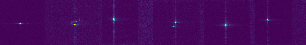
\includegraphics[width=0.8\textwidth]{training_data_example.png}
    \caption{Examples of delay-Doppler snapshots for different room occupancy scenarios.}
    \label{fig:snapshots}
\end{figure}

\section{Methodology}
The model development process involved data preprocessing, designing a CNN architecture, and hyperparameters optimization.

\subsection{Data Preprocessing}
The training data was loaded from PNG images and preprocessed by converting to RGB, cropping to remove white borders, resizing to a consistent dimension, and normalizing pixel values. The data was then split into training and validation sets.
Image augmentation techniques were explored in an attempt to improve model performance. Various augmentation methods, including rotation, flipping, and scaling, were applied to the training dataset to increase its diversity and robustness. However, despite these efforts, the accuracy value did not improve. This suggests that the original dataset may already contain sufficient variability for the model to learn effectively.

\subsection{Model used}
A CNN architecture was used for image classification. The model consists of multiple convolutional layers with ReLU activation, followed by max pooling, flattening, dense layers with ReLU activation, dropout regularization, and a final dense layer with softmax activation for multi-class classification (see Figure \ref{fig:architecture}). This model proved to yield a high accuracy value.

\begin{figure}
    \centering
    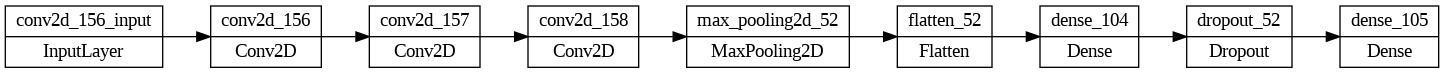
\includegraphics[width=1\textwidth]{model_plot.png}
    \caption{CNN architecture used for room occupancy classification.}
    \label{fig:architecture}
\end{figure}

\subsection{Hyperparameter Optimization}
Hyperparameter tuning was performed using Optuna to find the best combination of hyperparameters. The objective function defined the search space for the number of convolutional filters, dense units, dropout rate, and learning rate. Optuna optimized these hyperparameters based on the validation accuracy (see Figure \ref{fig:accuracy}).

\begin{figure}
    \centering
    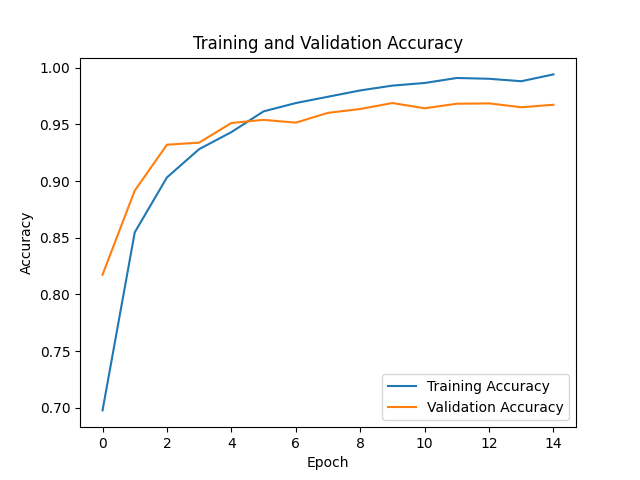
\includegraphics[width=0.7\textwidth]{accuracy_curves.png}
    \caption{Training and validation accuracy curves during model training.}
    \label{fig:accuracy}
\end{figure}

\section{Conclusion}
The CNN model, optimized using Optuna, achieved a high validation accuracy of 96.94\%. This work advances occupancy detection for applications in smart environments, security systems, and others. The source code is available on GitHub \textcolor{blue}{\href{https://github.com/Bitrey/MLBrno/blob/master/Project/Project.ipynb}{here}}.

\vspace*{\fill}

% \vspace{2em}
\hrulefill
\vspace{1em}

\textbf{Alessandro Amella \textcopyright{} 2024}

\end{document}